% Nome do capítulo
\chapter{Revisão de Literatura}
% Label para referenciar
\label{ch:revisao}

% Diminuir espaçamento entre título e texto
\vspace{-1.9cm}

% Texto do capítulo
Este capítulo apresenta uma visão geral das técnicas e tecnologias existentes que se relacionam com o tema do trabalho proposto. Foi feita uma pesquisa sobre braços e mãos robóticas, suas aplicações e tecnologias utilizadas, além de um estudo sobre luvas eletrônicas e sensores comumente adotados para seu funcionamento. Os trabalhos citados, e outros trabalhos relacionados, podem ser encontrados na Biblioteca Digital IEEE Xplore (\citeonline{ieee}) buscando pelos termos \textit{``robot arm''}, \textit{``data glove''} ou similares.

\section{Braços Robóticos}
\label{sec:brac}
Braços robóticos são máquinas programáveis compostas por articulações, construídas para a realização de tarefas repetitivas, desagradáveis ou perigosas \cite{occupational1996osha}. Possuem articulações análogas às existentes nos braços humanos, como ombros, cotovelos e pulsos. O atuador robótico (\textit{end effector}, em inglês) é a parte do robô, geralmente conectada ao pulso, que interage com o ambiente e seria equivalente à mão humana \cite{end_effect}. Outra característica importante dos braços robóticos é a quantidade de Graus de Liberdade (\ac{DOF}), ou seja, a quantidade de parâmetros independentes necessários para determinar a posição final do atuador. Nos próximos parágrafos serão apresentados trabalhos envolvendo braços robóticos, com o intuito de apresentar uma visão geral das tecnologias e técnicas utilizadas.

Existem aplicações comuns de braços robóticos para pintura, soldagem, rotação e transporte de peças. Os braços robóticos mais comuns utilizam garras como atuadores, pois são fáceis de fabricar e controlar, porém, isso limita a quantidade de movimentos que o robô pode realizar. Em certas aplicações, como na fabricação de próteses robóticas, é desejável que se tenha uma maior quantidade de \ac{DOF} no atuador para garantir maior similaridade com a mão humana.

De acordo com \citeonline{potkonjak1998redundancy}, o conjunto de mão e braço possui no total 26 \ac{DOF} (7 para o braço e 19 para a mão). Para a tarefa de escrita com um lápis, por exemplo, pode-se reduzir os \ac{DOF} da mão e do braço para 2 e 6, respectivamente, totalizando um mínimo de 8 \ac{DOF}, representados na Figura \ref{fig:dof}. O trabalho dos autores se foca em analisar o movimento de um braço antropomórfico na tarefa de escrita, elaborando um novo esquema de controle. Foi que para um certo nível de legibilidade, existe uma inclinação ideal das letras que resulta em um movimento mínimo dos dedos.

\begin{figure}[h]
  % Alterar espaçamentos antes e depois do caption
  \setlength{\abovecaptionskip}{0pt}
  \setlength{\belowcaptionskip}{0pt}
  % Caption
  \caption[Modelo de articulações do braço e mão]{Modelo de articulações do braço e mão}
  \centering
  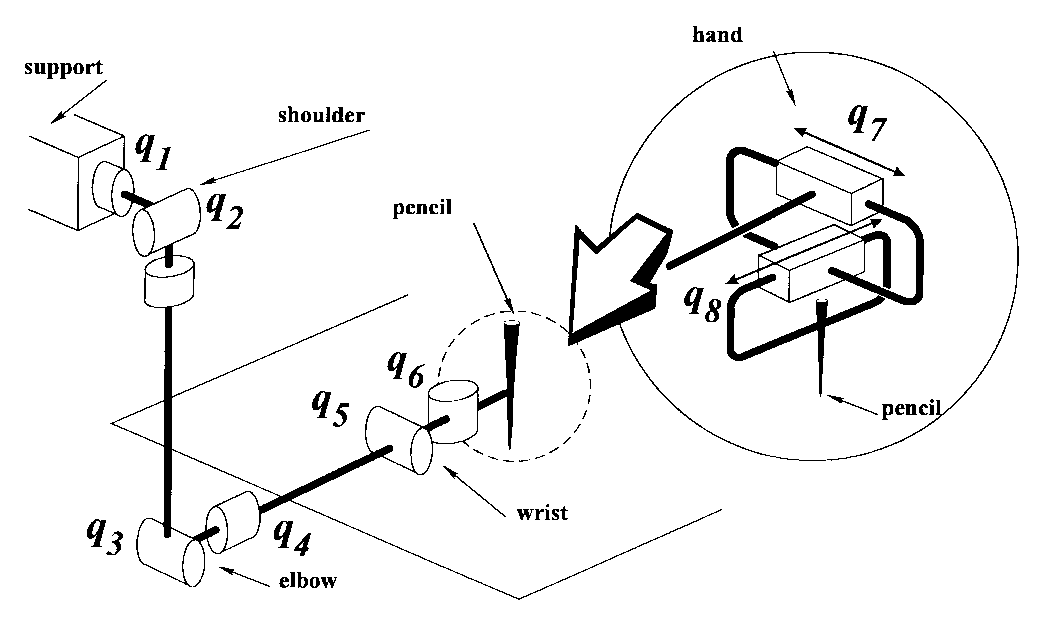
\includegraphics[width=.5\textwidth]{imagem/redundancy_dof}
  % Caption centralizada
  \captionsetup{justification=centering}
  \captionfont{\small{\textbf{\\Fonte: \citeonline{potkonjak1998redundancy}}}}
  \label{fig:dof}
\end{figure}

O trabalho realizado por \citeonline{sun2013calligraphy} descreve um robô com 6 \ac{DOF} denominado \textit{Callibot} (Figura \ref{fig:callibot}), capaz de escrever caracteres chineses utilizando um pincel. Os caracteres são ``ensinados'' gravando as posições de cada motor periodicamente enquanto uma pessoa escreve com o pincel e, em seguida, o robô reproduz os movimentos gravados. Os resultados obtidos foram satisfatórios, mostrando que \textit{Callibot} consegue reproduzir trabalhos complexos com estética agradável.

\begin{figure}[H]
  \setlength{\abovecaptionskip}{0pt}
  \setlength{\belowcaptionskip}{0pt}
  \caption[Callibot]{Callibot}
  \centering
  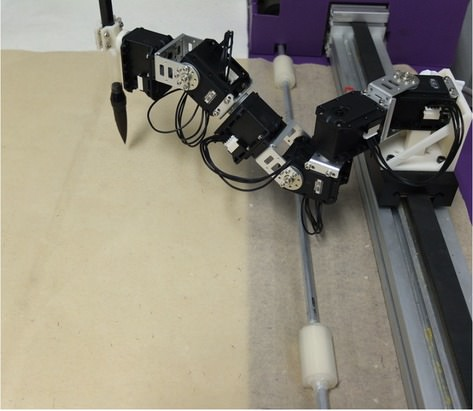
\includegraphics[width=.5\textwidth]{imagem/callibot}
  \captionsetup{justification=centering}
  \captionfont{\small{\textbf{\\Fonte: \citeonline{sun2013calligraphy}}}}
  \label{fig:callibot}
\end{figure}

O trabalho de \citeonline{xudesign} mostra o desenvolvimento de uma mão robótica, mostrada no Figura \ref{fig:antro_hand}, que tenta replicar partes biomecânicas importantes da mão, fazendo com que ela seja um réplica que possui características cinemáticas e dinâmicas similares. Os autores propõem que essa mão robótica possa ser utilizada para aplicações de manipulação remota de objetos, e possa ser integrada com sensores de toque na ponta dos dedos, além do poder servir como base para regeneração de membros e para pesquisas na área de neuroprostética\footnote{Área de pesquisa para desenvolvimento de próteses neurais. Uma prótese neural é um dispositivo que fornece ou recebe informações do sistema nervoso \cite{neuro}.}.

\begin{figure}[H]
  \setlength{\abovecaptionskip}{0pt}
  \setlength{\belowcaptionskip}{0pt}
  \caption[Mão antropomórfica]{Mão antropomórfica}
  \centering
  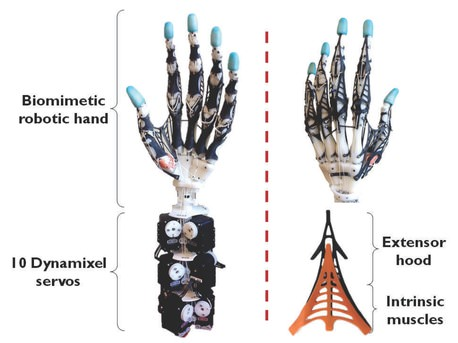
\includegraphics[width=.5\textwidth]{imagem/antro_hand}
  \captionsetup{justification=centering}
  \captionfont{\small{\textbf{\\Fonte: \citeonline{xudesign}}}}
  \label{fig:antro_hand}
\end{figure}

Em \citeonline{konnaris2016ethohand}, também foi desenvolvida uma mão robótica chamada de \textit{EthoHand} (Figura \ref{fig:etho_hand}). O dispositivo possui 24 \ac{DOF} e com articulação esférica no polegar, possibilitando movimentos naturais mais complexos para manipulação de objetos. A articulação funciona a partir de tendões conectados ao polegar e atuados por servomotores localizados externamente.

\begin{figure}[H]
  \setlength{\abovecaptionskip}{0pt}
  \setlength{\belowcaptionskip}{0pt}
  \caption[Detalhe da articulação esférica da EthoHand]{Detalhe da articulação esférica da EthoHand}
  \centering
  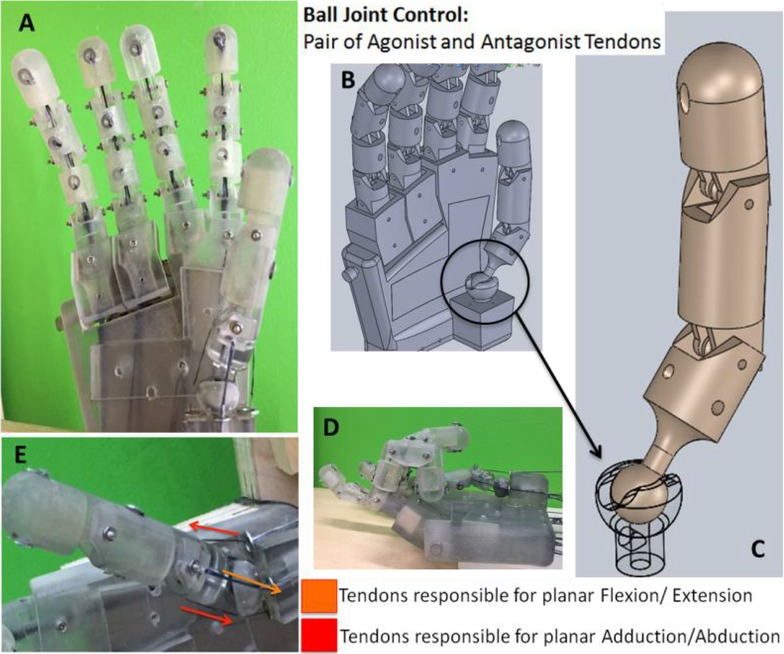
\includegraphics[width=.5\textwidth]{imagem/etho_hand}
  \captionsetup{justification=centering}
  \captionfont{\small{\textbf{\\Fonte: \citeonline{konnaris2016ethohand}}}}
  \label{fig:etho_hand}
\end{figure}

O trabalho de \citeonline{liu2008multisensory} apresenta uma mão robótica chamada de DLR/HIT HAND II (Figura \ref{fig:dex_hand}), com 5 dedos que possui sensores de posição, temperatura e força. Enquanto os outros trabalhos apresentados nessa seção utilizam motores externos que controlam tendões que movimentam os dedos, essa mão robótica utiliza motores e componentes eletrônicos que ficam no interior de cada dedo e da palma da mão para movimentá-los, tornando o produto final mais compacto e portável.

\begin{figure}[H]
  \setlength{\abovecaptionskip}{0pt}
  \setlength{\belowcaptionskip}{0pt}
  \caption[DLR/HIT HAND I e II]{DLR/HIT HAND I e II}
  \centering
  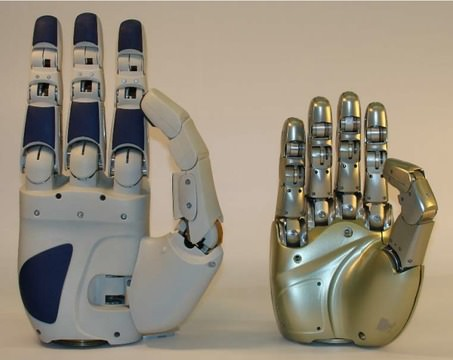
\includegraphics[width=.5\textwidth]{imagem/dex_hand}
  \captionsetup{justification=centering}
  \captionfont{\small{\textbf{\\Fonte: \citeonline{liu2008multisensory}}}}
  \label{fig:dex_hand}
\end{figure}

Para o controle de braços e mãos robóticas, principalmente as mais antropomórficas, é comum a utilização de luvas eletrônicas, como no trabalho de \citeonline{konnaris2016ethohand}, onde foi utilizada a \textit{CyberGlove} para controle remoto da mão robótica desenvolvida. Luvas eletrônicas são úteis pois possibilitam a replicação mais fiel de movimentos humanos além de permitir um controle mais intuitivo ao usuário.

\section{Luvas Eletrônicas (\textit{Data Gloves})}
\label{sec:luv}
Luvas eletrônicas (\textit{Data Gloves}) são dispositivos que utilizam sensores de movimento, como acelerômetros, giroscópios ou sensores de flexibilidade, para reconhecimento ou reprodução de gestos da mão humana \cite{kim20093}. Elas são utilizadas para, por exemplo, captura de movimentos das mãos para utilização em filmes, jogos digitais, reconhecimento de linguagem de sinais, controle de atuadores robóticos ou para \ac{IHC} e interação com ambientes de \ac{RV}.

De acordo com \citeonline{sturman1994survey}, a primeira luva eletrônica, a \textit{Sayre Glove} (Figura \ref{fig:sayre}) foi desenvolvida por Thomas DeFanti e Daniel Sandin na Universidade de Illinois em Chicago em 1976. Ela funcionava com tubos flexíveis que possuíam um emissor e um receptor de luz posicionados sobre os dedos e, conforme se flexionava, a quantidade de luz no receptor variava, gerando uma diferença de tensão que era medida e então usada como entrada para algum sistema. Na indústria do entretenimento, ainda segundo os autores, a fabricante de brinquedos \textit{Mattel} produziu em 1989 uma luva eletrônica de baixo custo chamada \textit{Power Glove}, que era usada como controle para alguns jogos da plataforma \textit{Nintendo}. Seu produto utilizava uma tinta resistiva que registrava o flexionamento dos dedos e um sensor acústico que captava a posição da mão no espaço com o auxílio de um emissor acústico instalado sobre a televisão. A tecnologia utilizada em luvas eletrônicas evoluiu bastante, contando com sensores mais precisos, novas técnicas de de captação de movimentos utilizando sensores de campo magnético \cite{fahn2005development} ou acelerômetros \cite{kim20093} e de cálculo de posicionamento no espaço utilizando sensores de luz infravermelha ou câmeras. A luva proposta nesse trabalho apresenta uma solução de baixo custo para captura de movimentos dos dedos e do pulso.

\begin{figure}[h]
  \setlength{\abovecaptionskip}{0pt}
  \setlength{\belowcaptionskip}{0pt}
  \caption[Sayre Glove]{Sayre Glove}
  \centering
  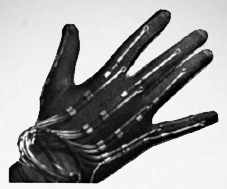
\includegraphics[width=.4\textwidth]{imagem/sayreGlove}
  \captionsetup{justification=centering}
  \captionfont{\small{\textbf{\\Fonte: \citeonline{sayre}}}}
  \label{fig:sayre}
\end{figure}

\begin{figure}[ht!]
  \centering
  % Alterar espaçamentos antes e depois do caption
  \setlength{\abovecaptionskip}{0pt}
  \setlength{\belowcaptionskip}{0pt}
  % Caption
  \caption[Exemplos de luvas eletrônicas]{Exemplos de luvas eletrônicas}
  \subfloat[5DT Data Glove Ultra]{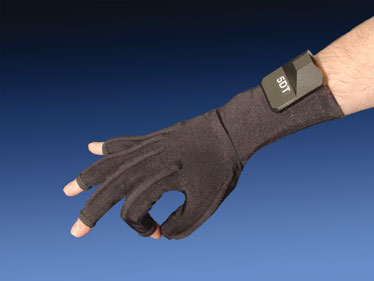
\includegraphics[height= 5cm]{imagem/5dtultra}\label{fig:5dt}}
  \quad
  \subfloat[Avatar VR]{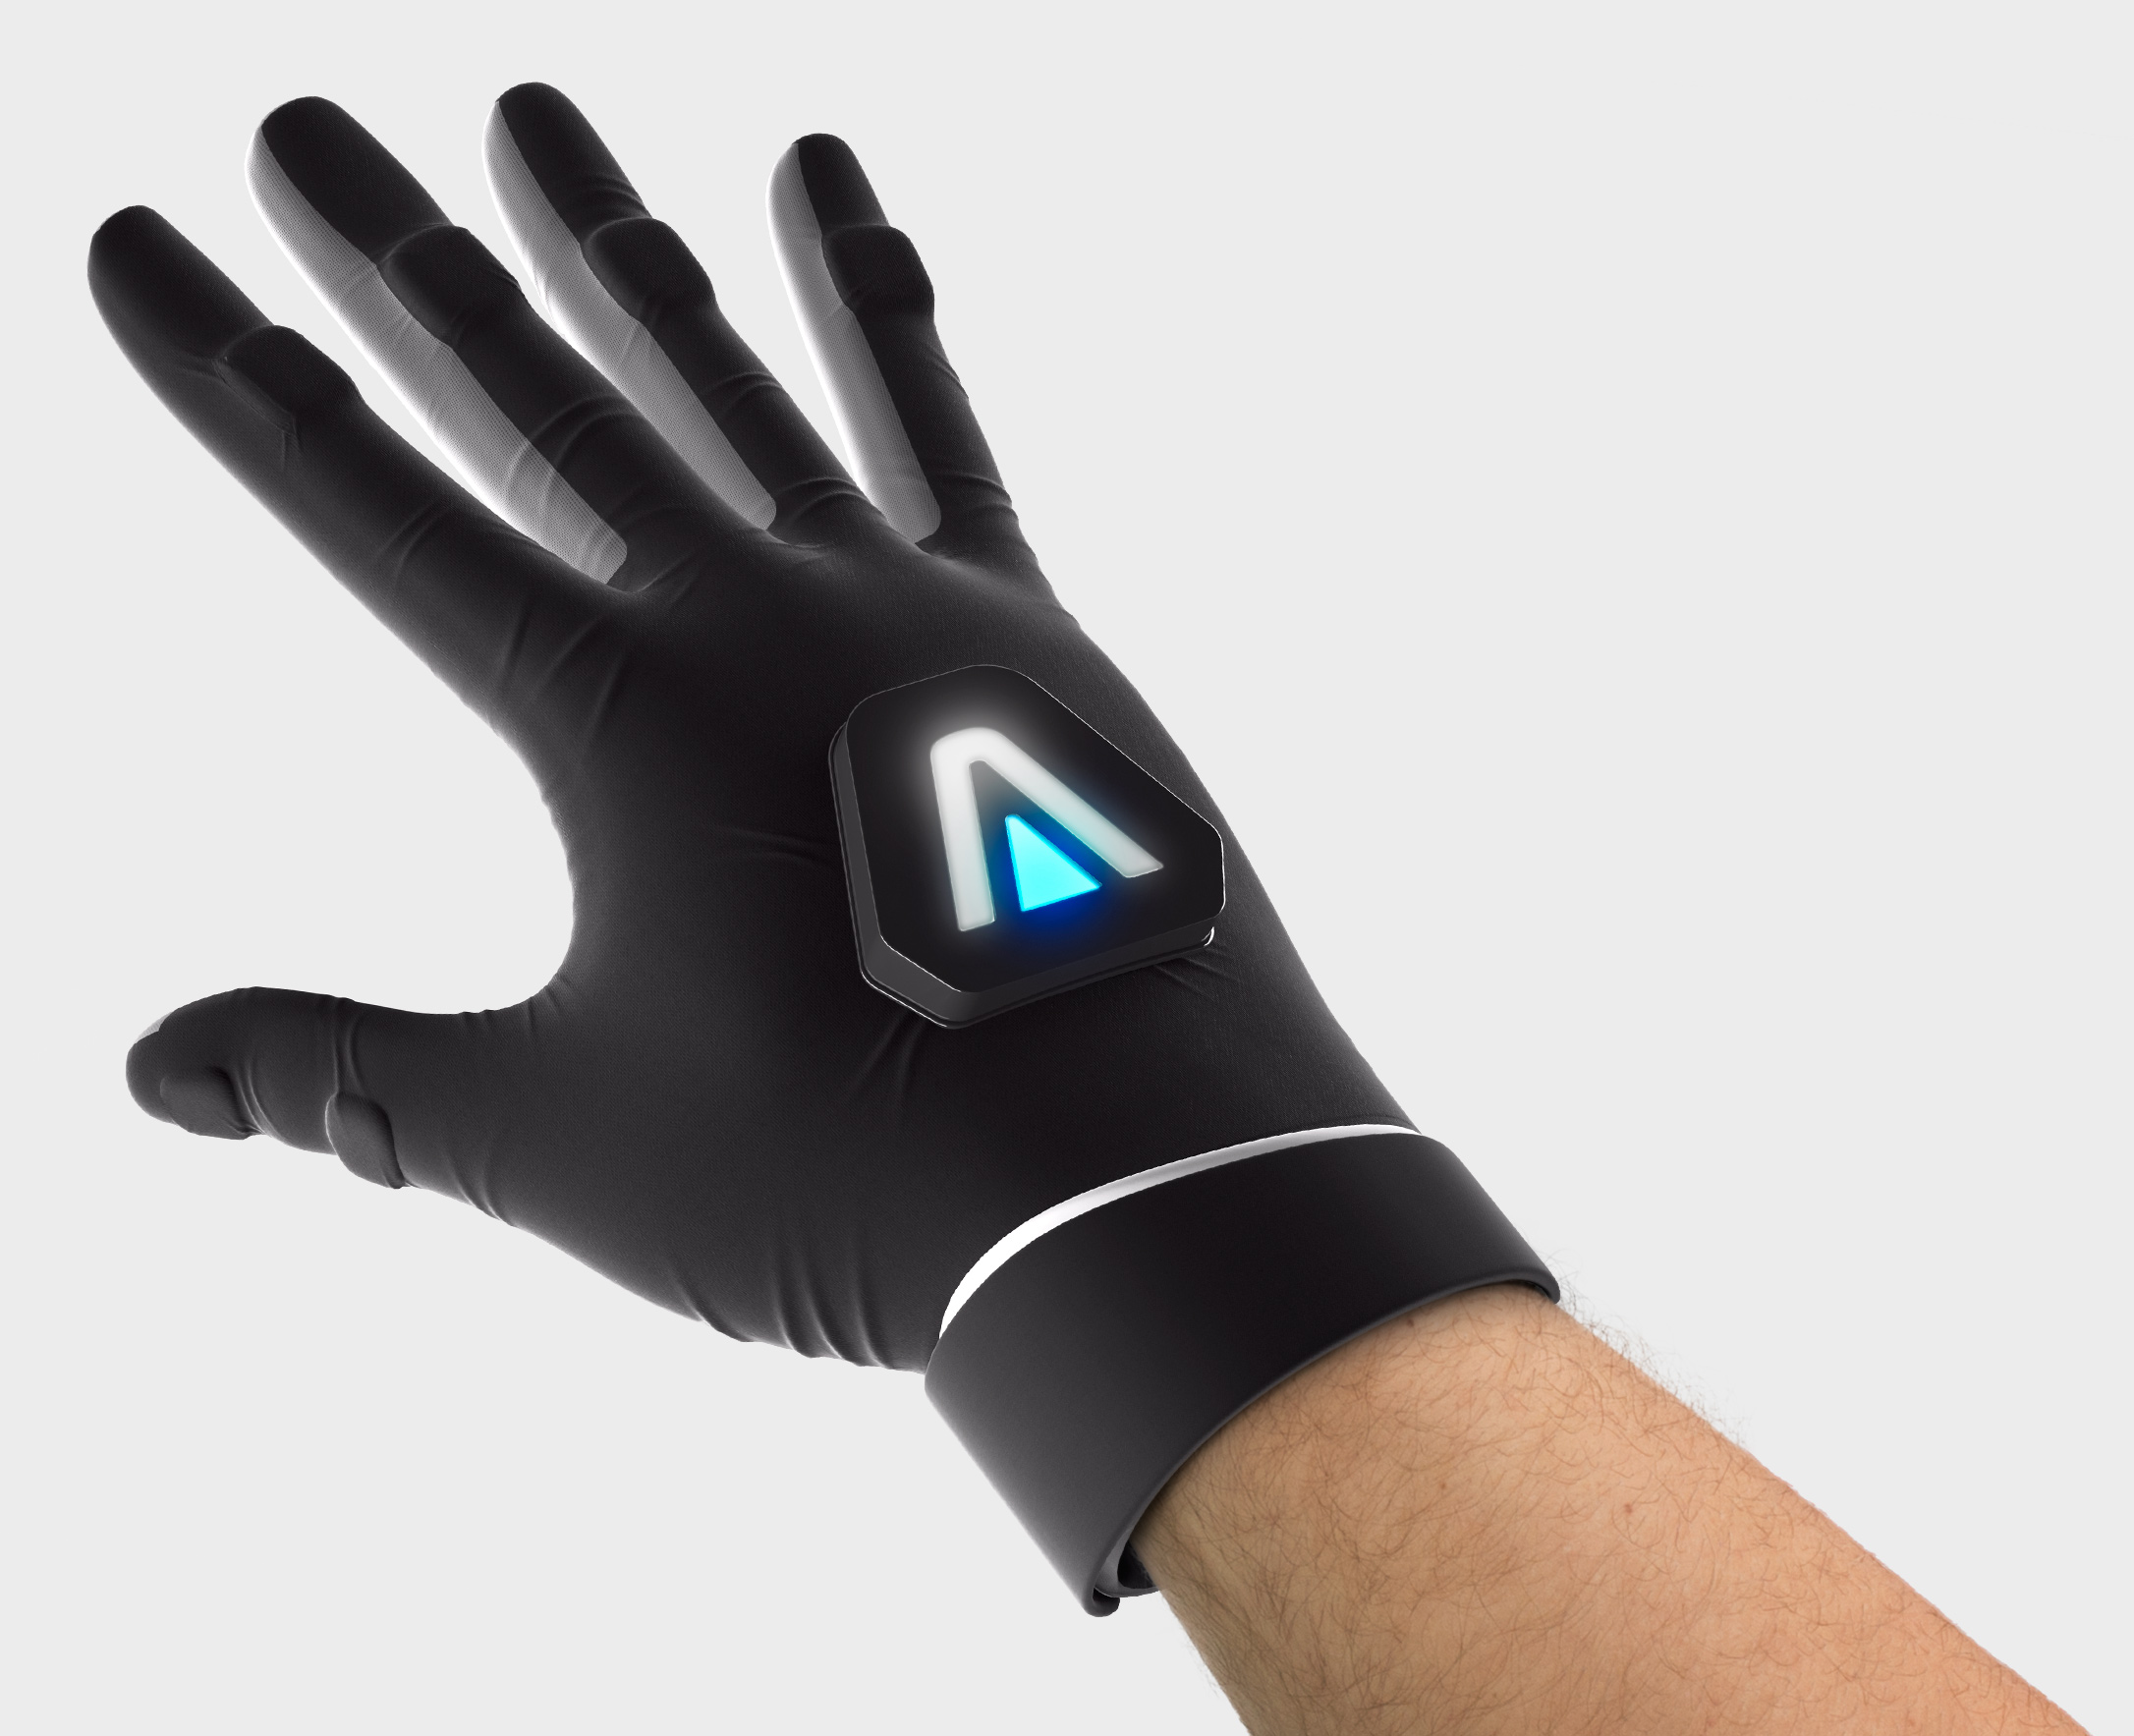
\includegraphics[height=5cm]{imagem/AvatarVR3}\label{fig:avatar}}
  \\
  \subfloat[Cyber Glove III]{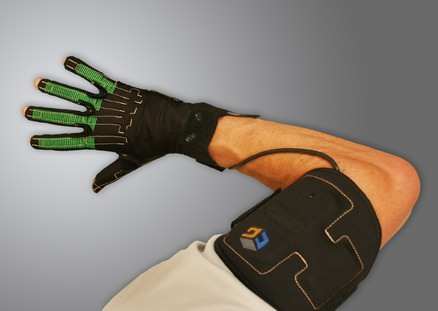
\includegraphics[height=5cm]{imagem/cg3p}\label{fig:cyberglove}}
  \quad
  \subfloat[Manus VR]{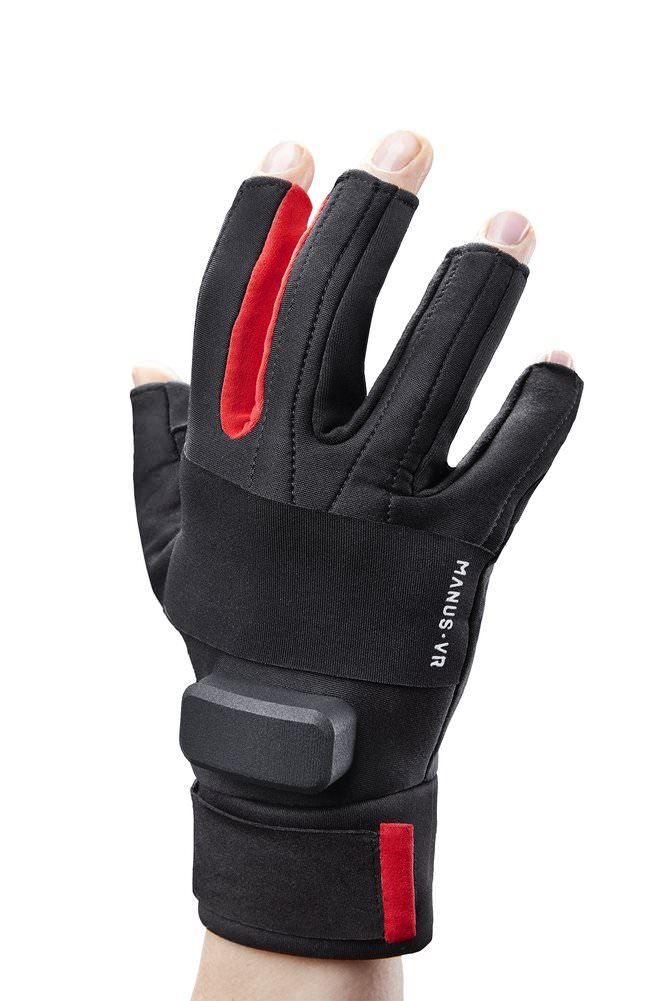
\includegraphics[height=5cm]{imagem/ManusVR}\label{fig:manus}}
  % Caption centralizada
  \captionsetup{justification=centering}
  \captionfont{\small{\textbf{\\Fontes:  \citeonline{5dt},
  \citeonline{avatar}, \citeonline{cyberglove}, \citeonline{manus}}}}
  \label{fig:luvas}
\end{figure}

A \textit{CyberGlove III} (Figura \ref{fig:cyberglove}) produzida pela \textit{CyberGlove Systems} é bastante utilizada em pesquisas acadêmicas, como por exemplo no trabalho realizado por \citeonline{perez2014objective}, que tinha por objetivo analisar a Ergonomia de cirurgiões ao realizar uma cirurgia de laparoscopia\footnote{``A laparoscopia é uma técnica de cirúrgica minimamente invasiva, na qual são utilizadas apenas pequenas incisões entre 0,5 e 1,0 cm para observar o interior da cavidade abdominal e os órgãos aí presentes.'' \cite{laparos}.}, capturando os movimentos do pulso e dos dedos dos cirurgiões. A \textit{5DT Data Glove 5 Ultra} (Figura \ref{fig:5dt}) produzida pela \textit{Fifth Dimensional Technologies} é outra luva eletrônica para utilização em captura de movimentos para animações realistas em tempo-real \cite{5dt}. Seu diferencial é o fato de utilizar sensores de fibra óptica para detectar o flexionamento dos dedos.

Atualmente, novas luvas eletrônicas estão sendo desenvolvidas com o objetivo de serem utilizadas em aplicações de \ac{RV} ou \ac{RA}\footnote{\ac{RV} diz respeito ao ambiente completamente virtual onde o usuário não tem contato com o mundo real. \ac{RA} permite que objetos virtuais sejam adicionados ao ambiente real \cite{azuma1997survey}}
. Dois exemplos notáveis são a \textit{Manus VR} (Figura \ref{fig:manus}) e a \textit{Avatar VR} (Figura \ref{fig:avatar}) que diferem das luvas citadas anteriormente pois, além de sensores de flexão, utilizam também as chamadas Unidades de Medição Inercial (\acf{IMU}). A Tabela \ref{tab:comp} mostra uma comparação entre os modelos de luvas citados nesta seção. Percebe-se que, dentre as luvas analisadas, a \textit{5DT Data Glove Ultra} é a única que utiliza sensores baseados em fibra ótica, com um sensor por dedo. Também nota-se que o preço da \textit{Cyber Glove III} é o mais caro entre eles\footnote{Preço informado pelo fornecedor}, devido à sua grande quantidade de sensores utilizados, sendo 13 vezes mais cara que a 5DT Data Glove Ultra.

\begin{table}[H]
    \centering
    \footnotesize
    \setlength{\abovecaptionskip}{0pt}
    \setlength{\belowcaptionskip}{0pt}
    \caption[Comparação entre modelos de luvas eletrônicas]{Comparação entre modelos de luvas eletrônicas}
    \label{tab:comp}
    \begin{tabularx}{\textwidth}{p{3.7cm}XXrr}
      \hline\hline
      \multicolumn{1}{c}{Luvas} & \multicolumn{1}{c}{Interface} & \multicolumn{1}{c}{Tipo de Sensor} & \multicolumn{1}{c}{Nº de Sensores} & \multicolumn{1}{c}{Preço por Mão}\\
      \hline
      5DT Data Glove 5 Ultra    & USB                           & Fibra óptica                       & 5                                  & US\$995\\
      Avatar VR                 & WiFi                          & \ac{IMU}                           & 6                                  & \euro{1100}\\
      CyberGlove III            & WiFi e USB                    & Flexão                             & 18 ou 22                           & US\$12995\\
      Manus VR                  & WiFi                          & \ac{IMU}/Flexão                    & 1 \ac{IMU} + 5 Flexão              & US\$250\\
      \hline \hline
    \end{tabularx}
    \\\vspace{1.3mm}
    \captionfont{\small{\textbf{Fontes: \citeonline{5dt}, \citeonline{avatar}, \citeonline{cyberglove}, \citeonline{manus}, \citeonline{manus_specs}}}}
  \end{table}

Uma das grandes dificuldades na evolução de luvas eletrônicas está na grande quantidade de movimentos que podem ser exercidos pela mão humana, tornando complexa a sua captação e reprodução fiel por computadores ou braços robóticos. Outro fator limitante é o alto custo dos dispositivos utilizados para a fabricação de luvas eletrônicas, sendo necessários sensores com alta precisão e repetibilidade, além de serem compactos e leves a fim de não limitar os movimentos do usuário final.

\section{Sensores}
\label{sec:sens}
Um sensor é ``um dispositivo que detecta mudanças em um estímulo físico e as transformam em um sinal que pode ser medido ou gravado.''\cite{sensor}\footnote{``[\ldots] a device that detects a change in a physical stimulus and turns it into a signal which can be measured or recorded [\ldots]''}. Os sensores utilizados em luvas eletrônicas podem ser:
\begin{enumerate}
\item[a)] flexão -- mede deformações (dobras) em sua superfície. São utilizados para detectar o movimento de flexão e extensão dos dedos;
\item[b)] acelerômetro -- mede a aceleração física exercida sobre ele. São utilizados para detectar a rotação da mão no espaço.
\end{enumerate}

\subsection{Sensor de flexão baseado em tinta resistiva}
\label{subsec:flextin}

Estes são sensores passivos que possuem uma camada de tinta resistiva sobre uma tira de plástico flexível (Figura \ref{fig:flextinta}). Quando o sensor está plano (Figura \ref{fig:plano}), ele possui um valor de resistência elétrica, e, quando flexionado (Figura \ref{fig:curvo}), as partículas condutivas da tinta se afastam, dificultando a passagem de elétrons, aumentando sua resistência.

\begin{figure}[H]
  \centering
  % Alterar espaçamentos antes e depois do caption
  \setlength{\abovecaptionskip}{0pt}
  \setlength{\belowcaptionskip}{0pt}
  % Caption
  \caption[Funcionamento do sensor de flexão]{Funcionamento do sensor de flexão}
    \subfloat[Partículas condutivas próximas]{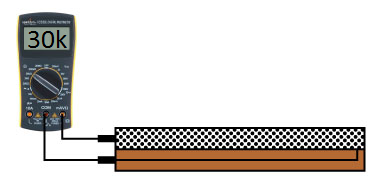
\includegraphics[width=.5\textwidth]{imagem/sensor_reto}\label{fig:plano}}\\
    \subfloat[Partículas condutivas afastadas]{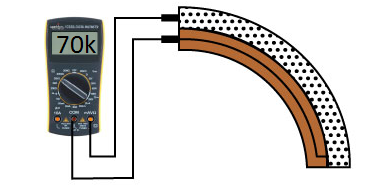
\includegraphics[width=.5\textwidth]{imagem/sensor_curvo}\label{fig:curvo}}
  % Caption centralizada
  \captionsetup{justification=centering}
  \captionfont{\small{\textbf{\\Fontes: \citeonline{sparkflex}}}} 
  \label{fig:sensorflex}
\end{figure}

\begin{figure}[H]
  \setlength{\abovecaptionskip}{0pt}
  \setlength{\belowcaptionskip}{0pt}
  \caption[Sensor de flexão baseado em tinta resistiva]{Sensor de flexão baseado em tinta resistiva}
  \centering
  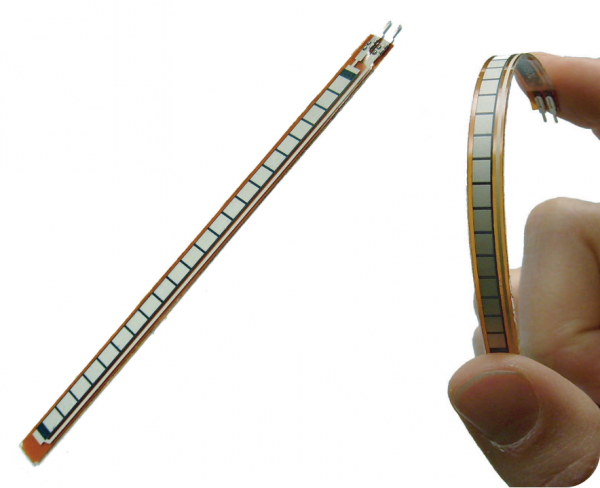
\includegraphics[width=.4\textwidth]{imagem/flexsensordirection}
  \captionsetup{justification=centering}
  \captionfont{\small{\textbf{\\Fonte: \citeonline{symbol2012flex}}}}
  \label{fig:flextinta}
\end{figure}

\subsection{Sensor de flexão baseado em fibra ótica}
\label{subsec:flexotic}
Os sensores baseados em fibra ótica (Figura \ref{fig:flexotico}) possuem um emissor de luz em uma extremidade e um receptor em outra. Quando o sensor é flexionado, a intensidade de luz que chega no receptor é diminuída devido às reflexões que ocorrem no interior da fibra ótica. Essa diferença de intensidade é medida e indica quanto o sensor foi flexionado.

\begin{figure}[H]
  \setlength{\abovecaptionskip}{0pt}
  \setlength{\belowcaptionskip}{0pt}
  \caption[Sensor de flexão baseado em fibra ótica]{Sensor de flexão baseado em fibra ótica}
  \centering
  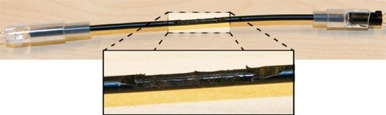
\includegraphics[width=.5\textwidth]{imagem/twend-optical}
  \captionsetup{justification=centering}
  \captionfont{\small{\textbf{\\Fonte: \citeonline{herkenrath2008twend}}}}
  \label{fig:flexotico}
\end{figure}

\subsection{\acf{IMU}}
\label{subsec:imu}
\ac{IMU}s são dispositivos que utilizam uma combinação de acelerômetros, giroscópios e, em alguns casos, magnetômetros para medir as diferentes forças que atuam sobre esse sensor, como aceleração, rotação ou campo magnético. Um \ac{IMU} consegue detectar translação e rotação em cada um dos eixos $X$, $Y$ e $Z$, totalizando 6 \ac{DOF} (Figura \ref{fig:imu}). 

\begin{figure}[H]
  \setlength{\abovecaptionskip}{0pt}
  \setlength{\belowcaptionskip}{0pt}
  \caption[Eixos de detecção de um \ac{IMU}]{Eixos de detecção de um \ac{IMU}}
  \centering
  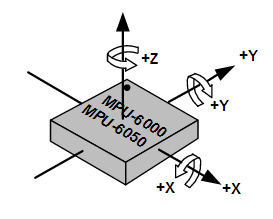
\includegraphics[width=.4\textwidth]{imagem/IMU_eixos}
  \captionsetup{justification=centering}
  \captionfont{\small{\textbf{\\Fonte: \citeonline{IMU}}}}
  \label{fig:imu}
\end{figure}

\subsubsection{Acelerômetro}
\label{subsubsec:accel}
Acelerômetros são dispositivos que medem a intensidade da força de aceleração exercida sobre ele. Geralmente possuem uma massa móvel suspensa por molas e, ao movimentar o dispositivo, a massa se desloca, deformando as molas e gerando um sinal elétrico que é medido para informar em que direção e com qual intensidade ocorreu a aceleração. Por exemplo, um acelerômetro em descanso na superfície da Terra medirá uma aceleração de aproximadamente \SI{9.81}{m/s^{2}} sobre o eixo $Z$, ou seja, a aceleração da gravidade. Acelerômetros detectam movimentos de translação nos eixos $X$, $Y$ e $Z$ do espaço, por isso possui 3 \ac{DOF} (Figura \ref{fig:accel}).

\begin{figure}[H]
  \setlength{\abovecaptionskip}{0pt}
  \setlength{\belowcaptionskip}{0pt}
  \caption[Estrutura do acelerômetro]{Estrutura do acelerômetro}
  \centering
  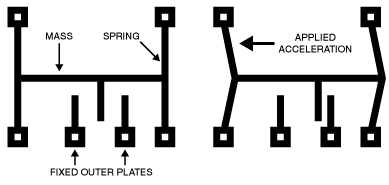
\includegraphics[width=.4\textwidth]{imagem/accel}
  \captionsetup{justification=centering}
  \captionfont{\small{\textbf{\\Fonte: \citeonline{accel}}}}
  \label{fig:accel}
\end{figure}

\subsubsection{Giroscópio}
\label{subsubsec:gyro}
Giroscópios detectam a rotação em torno de cada um dos eixos $X$, $Y$ e $Z$, ou seja, a velocidade angular ou a taxa de variação do ângulo de rotação em graus por segundo (\SI[per-mode=symbol]{}{\degree\per\second}). Existem três tipos básicos de giroscópios: Rotatórios, Ópticos e Vibratórios \cite{fraden2004handbook}, sendo este último o mais comum em circuitos integrados, pois tem menor tamanho em relação aos outros tipos. Eles possuem uma massa conectada por molas a uma estrutura, que por sua vez está conectada a uma segunda estrutura fixa no circuito (Figura \ref{fig:gyro}) . A massa central oscila verticalmente e, quando o giroscópio é submetido a uma rotação, a estrutura se move na horizontal, devido à força inercial de Coriolis\footnote{``A força de Coriolis é uma força que surge num sistema referencial em rotação que tende a alterar a trajetória dos corpos em movimento.'' \cite{coriolis}}. Como o giroscópio não possui uma referência fixa para suas medições, ele é suscetível a erros cumulativos ao longo do tempo, conforme sua utilização ou temperatura.

\begin{figure}[H]
  \setlength{\abovecaptionskip}{0pt}
  \setlength{\belowcaptionskip}{0pt}
  \caption[Estrutura do giroscópio]{Estrutura do giroscópio}
  \centering
  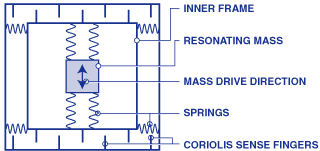
\includegraphics[width=.4\textwidth]{imagem/gyro_vsg1}
  \captionsetup{justification=centering}
  \captionfont{\small{\textbf{\\Fonte: \citeonline{gyroscope}}}}
  \label{fig:gyro}
\end{figure}

\subsubsection{Magnetômetro}
\label{subsubsec:mag}
Magnetômetros são sensores que detectam o efeito de Hall\footnote{ o efeito de Hall se refere ao desvio da trajetória normal das cargas fluindo em um semicondutor, quando este é submetido à ação de um campo magnético. Este desvio causa uma diferença de potencial que pode ser medida perpendicularmente ao sentido do movimento da corrente.\cite{hall}} (Figura \ref{fig:mag}). Quando a \ac{IMU} utiliza um magnetômetro, é possível detectar a intensidade do campo magnético em torno do dispositivo.

\begin{figure}[H]
  \setlength{\abovecaptionskip}{0pt}
  \setlength{\belowcaptionskip}{0pt}
  \caption[Demonstração do Efeito de Hall]{Demonstração do Efeito de Hall}
  \centering
  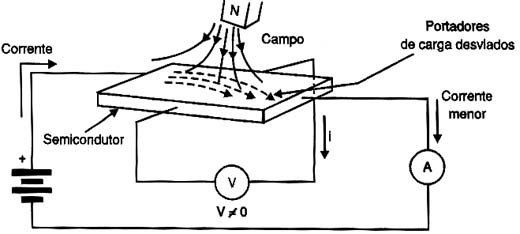
\includegraphics[width=.4\textwidth]{imagem/hall}
  \captionsetup{justification=centering}
  \captionfont{\small{\textbf{\\Fonte: \citeonline{hall}}}}
  \label{fig:mag}
\end{figure}

Nas \ac{IMU}s, os dados do acelerômetro, giroscópio e magnetômetro geralmente são usados em conjunto para fornecer leituras de orientação precisas, já que os dados do acelerômetro são muito ruidosos, o giroscópio é suscetível a erros cumulativos e o magnetômetro sofre interferência de campos magnéticos externos. As leituras suaves do giroscópio são combinadas com as do acelerômetro para reduzir ruídos, e as leituras do magnetômetro são usadas para detectar o campo magnético da Terra, sendo este usado como referência para calcular a orientação e também para corrigir os erros provenientes do giroscópio.%

\section{Trabalhos Relacionados}%
\label{sec:trabrel}%
Em \citeonline{fang2015robotic}, foi proposta uma luva eletrônica  composta de 18 \ac{IMMU} para controle remoto de um braço robótico. Dos \ac{IMMU} utilizados, 15 foram acoplados em cada um dos segmentos dos dedos, um na palma da mão, um no antebraço e um no braço (Figura \ref{fig:2015luva}). O robô controlado pela luva possui braço com 7 \ac{DOF}, mão com 4 \ac{DOF} e os dados das \ac{IMMU} foram mapeados em cada segmento do robô, de modo que as informações geradas pelas \ac{IMMU} são convertidas em instruções para controle do braço e da mão robótica (Figura \ref{fig:2015robo}). O primeiro teste executado foi para verificar o funcionamento correto da luva e das informações geradas, resultando em um erro médio quadrado das orientações no eixos $X$, $Y$ e $Z$ de menos de \ang{0.5}. Os próximos testes consistiram em controlar a mão e o braço robótico remotamente (Figura \ref{fig:2015controle}), mostrando que os movimentos realizados foram suaves e imitavam o movimento do braço do operador. Este trabalho mostra que, dado um sistema de captura adequado, é possível mapear os movimentos realizados por um humano em instruções de movimento de robôs através da utilização de sensores. Esse tipo de controle permite que braços robóticos sejam operados intuitivamente e com movimentos naturais. Entretanto, essa solução prioriza a captura do braço e antebraço e não os movimentos específicos da mão, que são necessários para o problema proposto nesse trabalho.

\begin{figure}[h]
  \centering
  \setlength{\abovecaptionskip}{0pt}
  \setlength{\belowcaptionskip}{0pt}
  \caption[Luva e Robô desenvolvidos por \citeonline{fang2015robotic}]{Luva e Robô desenvolvidos por \citeonline{fang2015robotic}}
    \subfloat[Luva]{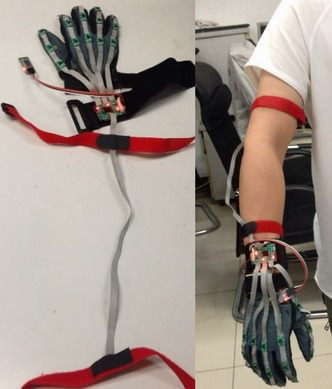
\includegraphics[height=5cm]{imagem/2015luva}\label{fig:2015luva}}
    \quad
    \subfloat[Robô]{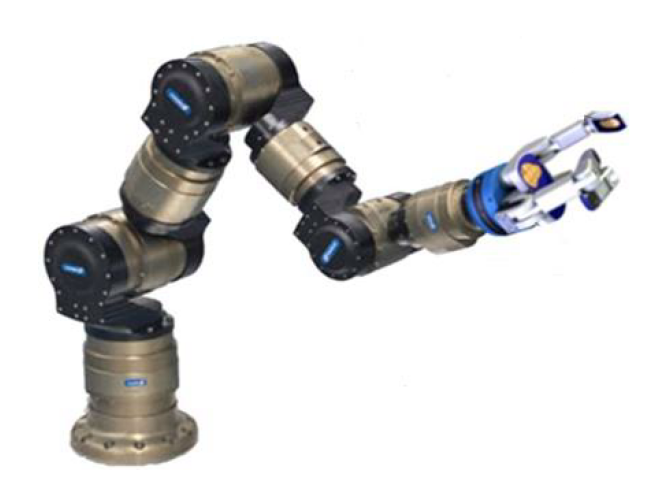
\includegraphics[height=5cm]{imagem/2015robo}\label{fig:2015robo}}\\
    \subfloat[Controle do Robô com a Luva]{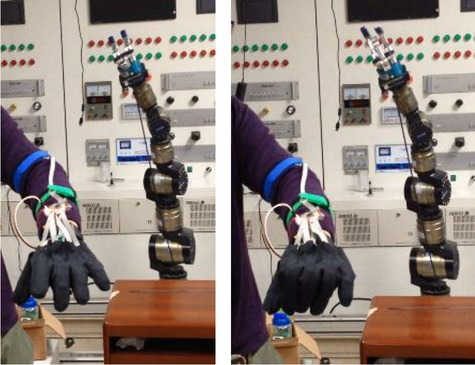
\includegraphics[width=.5\textwidth]{imagem/2015controle}\label{fig:2015controle}}
  \captionsetup{justification=centering}
  \captionfont{\small{\textbf{\\Fontes: \citeonline{fang2015robotic}}}}
  \label{fig:fang}
\end{figure}

Em \citeonline{fahn2005development}, foi desenvolvida uma luva eletrônica utilizando bobinas de indução magnética como sensores de movimento dos dedos. Utilizou-se três bobinas por dedo, duas geradoras de campo magnético e uma para medir a variação desse campo. Elas foram posicionadas sob os dedos, na região palmar (Figura \ref{fig:magneto}), para que o sinal da força eletromotriz, gerada pela variação do campo magnético, fosse grande o suficiente para se realizar as medições com precisão. Os autores ainda propuseram um método de calibração da luva que consistia em dois movimentos simples, sendo o primeiro com a mão aberta com os dedos esticados, e o segundo, com a mão fechada segurando um cilindro de modo que os ângulos formados com a primeira falange fossem de aproximadamente \ang{90}. Para prevenir interferências entre as bobinas, foi definido um tempo de ativação para cada bobina geradora, no qual o resultado das bobinas receptoras era detectado e enviado para um conversor \ac{A/D} que enviava os sinais para um microcontrolador para o processamento. Este método para captura do movimento dos dedos, embora preciso, é complexo computacionalmente devido aos cálculos envolvidos para obter os ângulos de dobra dos dedos. Além disso, este método é sensível à interferência de campos magnéticos exteriores.

\begin{figure}[H]
  \setlength{\abovecaptionskip}{0pt}
  \setlength{\belowcaptionskip}{0pt}
  \caption[Posicionamento das bobinas sensoras e geradoras]{Posicionamento das bobinas sensoras e geradoras}
  \centering
  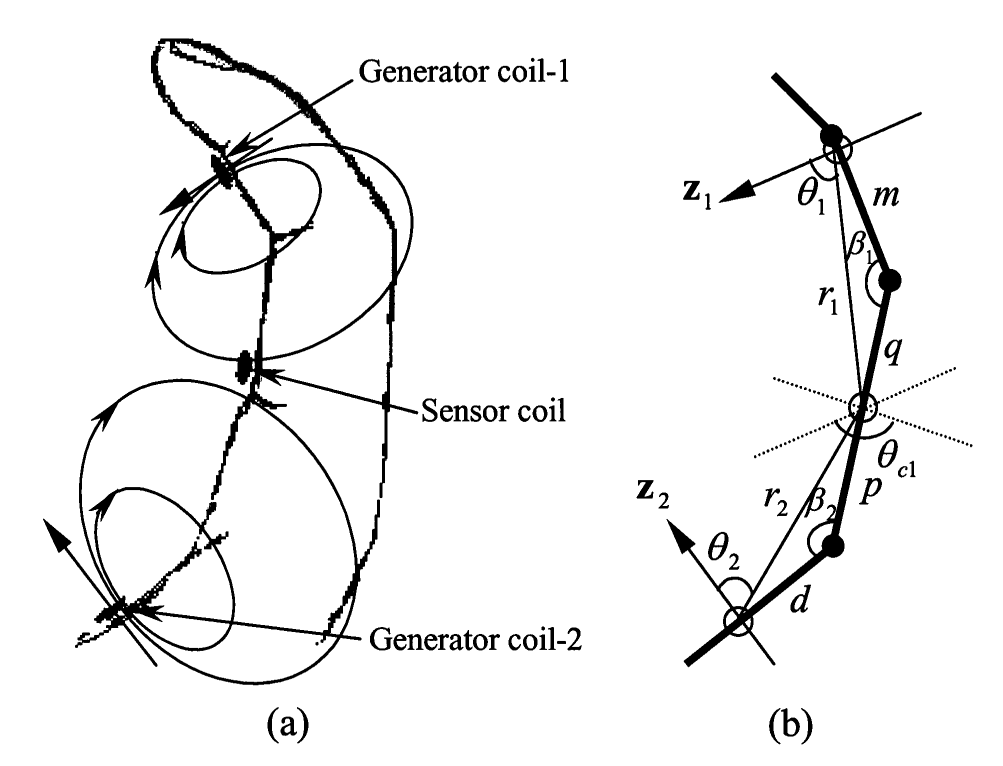
\includegraphics[width=.5\textwidth]{imagem/2005magneto}
  \captionsetup{justification=centering}
  \captionfont{\small{\textbf{\\Fonte: \citeonline{fahn2005development}}}}
  \label{fig:magneto}
\end{figure}


No trabalho de \citeonline{kim20093}, foi criada uma luva para reconhecimento de gestos utilizando três acelerômetros com 3 \ac{DOF} denominada \textit{KHU-1}. Um dos acelerômetros foi posicionado na região dorsal da mão para detectar sua orientação espacial, outro posicionado no polegar e o último posicionado no dedo médio, controlando os movimentos dos dedos indicador, médio, anelar e mínimo (Figura \ref{fig:2009accel}). A comunicação com o computador foi feita através de \textit{Bluetooth} para controlar um modelo \ac{3D} da mão. Os testes para reconhecimento de gestos consistiram na realização dos movimentos de ``pedra'', ``papel'' e ``tesoura'', com a mão na vertical, horizontal com palma para baixo e horizontal com palma para cima. A luva obteve taxa de acerto total no reconhecimento desses gestos, porém os autores não detalharam os procedimentos utilizados para validação dos testes. Uma das desvantagens desse projeto é que não há independência entre os dedos já que todos são controlados pelo dedo médio.

\begin{figure}[H]
  \setlength{\abovecaptionskip}{0pt}
  \setlength{\belowcaptionskip}{0pt}
  \caption[A luva \textit{KHU-1}]{A luva \textit{KHU-1}}
  \centering
  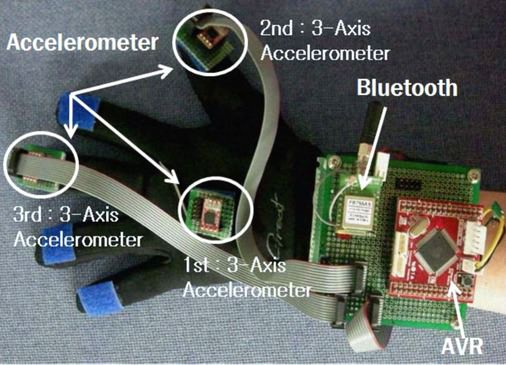
\includegraphics[width=.5\textwidth]{imagem/2009accel}
  \captionsetup{justification=centering}
  \captionfont{\small{\textbf{\\Fonte: \citeonline{kim20093}}}}
  \label{fig:2009accel}
\end{figure}

\citeonline{li2009smartglove} apresenta o desenvolvimento de uma luva eletrônica chamada \textit{SmartGlove} e de um \textit{encoder} linear ótico para detectar o ângulo de dobra de múltiplas articulações dos dedos (Figura \ref{fig:2009smartglove}). Os \textit{encoders} foram construídos com base em sensores de \textit{mouse} ótico e foram conectados a uma fita fixa na região dorsal da mão, que se deslocava sob os dedos quando eles se articulavam, possibilitando que um microcontrolador calculasse o ângulo dessa articulação baseado no movimento da fita detectado pelo sensor. A luva produzida possuía baixo custo devido aos materiais utilizados, fornecendo sensores com boa linearidade (\SI{99.4}{\percent} quando o dedo era dobrado) e precisão (menos de \ang{1} comparado ao acelerômetro), sendo leve e não intrusiva ao usuário. Os testes de verificação de linearidade e precisão dos sensores realizados pelo autor podem ser adotados para as luvas que detectam o ângulo de dobra das articulações, como é o caso da luva proposta neste trabalho.

\begin{figure}[H]
  \setlength{\abovecaptionskip}{0pt}
  \setlength{\belowcaptionskip}{0pt}
  \caption[Princípio de funcionamento da \textit{SmartGlove}]{Princípio de funcionamento da \textit{SmartGlove}}
  \centering
  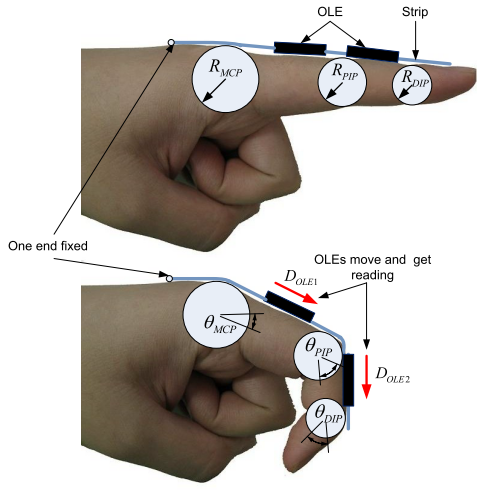
\includegraphics[width=.5\textwidth]{imagem/2009smartglove}
  \captionsetup{justification=centering}
  \captionfont{\small{\textbf{\\Fonte: \citeonline{li2009smartglove}}}}
  \label{fig:2009smartglove}
\end{figure}

O projeto de \citeonline{leap} é um dispositivo que utiliza giroscópios em conjunto com o \textit{Leap Motion}, que é um sensor que detecta movimentos no espaço, para criar um controle de \ac{RV} que é simples e não intrusivo. O sensor \textit{Leap Motion} fica afixado em um \textit{display} de \acl{RV} capturando os movimentos das mãos do usuário e, o giroscópio fica preso na palma da mão do usuário junto com dois botões para interação com o ambiente virtual (Figura \ref{fig:leap}). O projeto ainda está em desenvolvimento, mas se mostra uma técnica interessante para captura do movimentos e da orientação da mão em ambientes \ac{3D}.

\begin{figure}[H]
  \setlength{\abovecaptionskip}{0pt}
  \setlength{\belowcaptionskip}{0pt}
  \caption[Controle de \ac{RV}]{Controle de \ac{RV} de \citeonline{leap}}
  \centering
  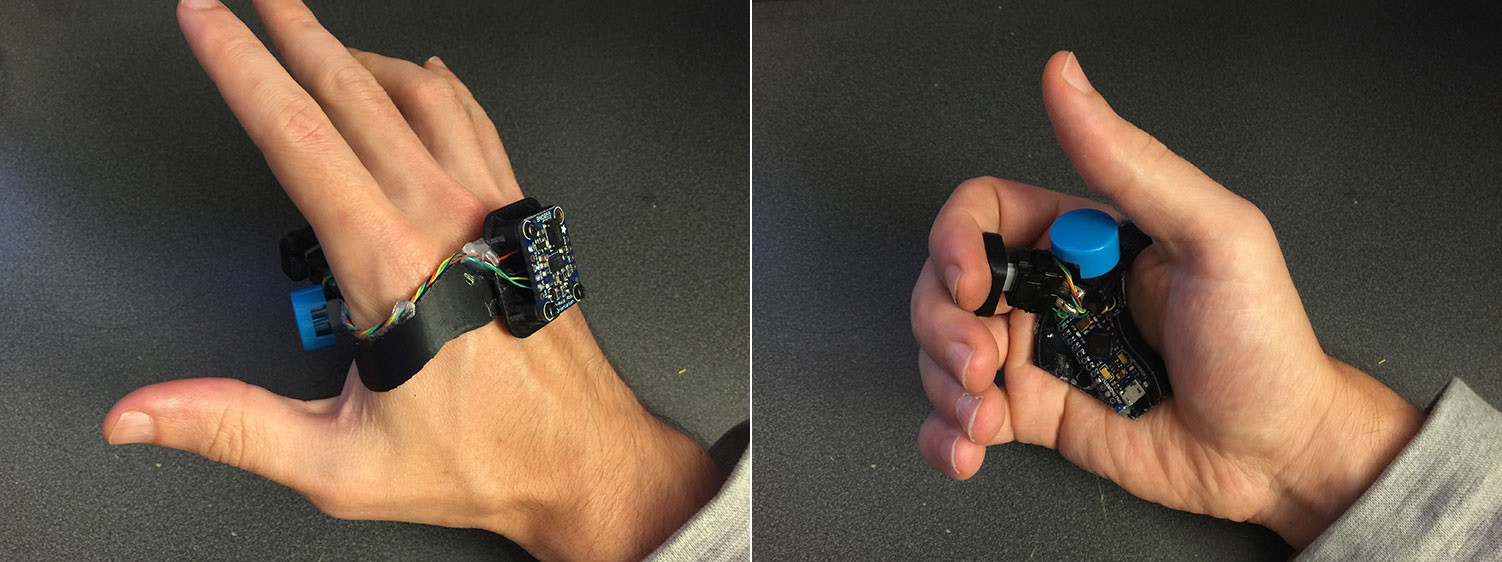
\includegraphics[height=4.5cm]{imagem/leap}
  \captionsetup{justification=centering}
  \captionfont{\small{\textbf{\\Fonte: \citeonline{leap}}}}
  \label{fig:leap}
\end{figure}

O presente trabalho baseia-se na continuidade do trabalho de \citeonline{roversi}, que consistiu no desenvolvimento de um protótipo de luva eletrônica de baixo custo, utilizando sensores de flexão baseados em tinta resistiva para detecção do movimento dos dedos, e uma \ac{IMU} para detecção da orientação da mão, acoplados à plataforma Arduino (Figura \ref{fig:luvaroversi}). No trabalho do autor, foram utilizados dois sensores de flexão em cada dedo a fim de detectar a articulação da primeira falange independentemente das articulações da segunda e terceira falanges. Para os testes, foi modelada uma mão \ac{3D} no ambiente de desenvolvimento de jogos \citeonline{unity}, e os movimentos realizados pelo usuário deveriam ser reproduzidos na mão virtual. Um dos problemas dessa luva foi o fato de ela não reproduzir movimentos de adução e abdução dos dedos ou de desvio radial e ulnar do pulso.

\begin{figure}[H]
  \setlength{\abovecaptionskip}{0pt}
  \setlength{\belowcaptionskip}{0pt}
  \caption[A luva de \citeonline{roversi}]{A luva de \citeonline{roversi}}
  \centering
  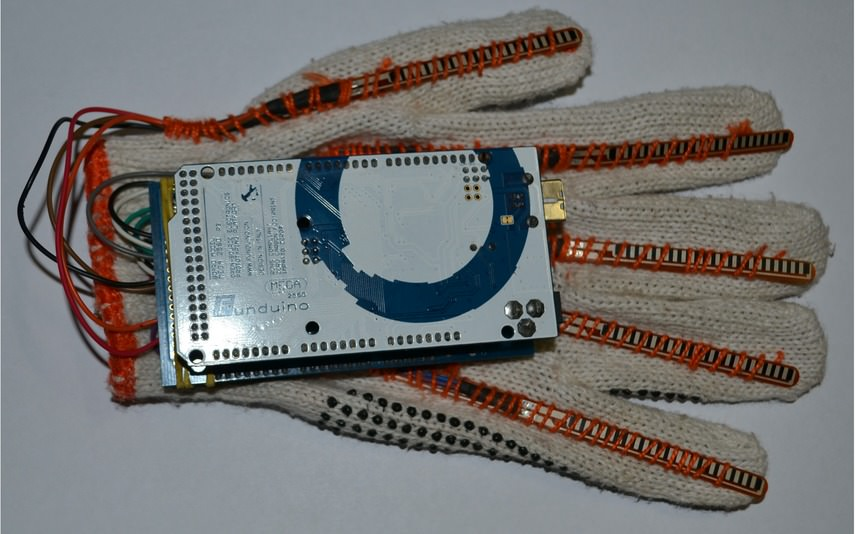
\includegraphics[width=.5\textwidth]{imagem/2016roversi}
  \captionsetup{justification=centering}
  \captionfont{\small{\textbf{\\Fonte: \citeonline{roversi}}}}
  \label{fig:luvaroversi}
\end{figure}
